\documentclass[11pt]{article}
% Packages
\usepackage{times}
\usepackage[fleqn]{amsmath}
\usepackage{amssymb}
\usepackage{anysize}
\usepackage{graphicx}
\usepackage{booktabs}
\usepackage{titlesec}
\usepackage{float}
\usepackage{natbib}
\usepackage[english]{babel}
\usepackage[autolanguage]{numprint}
\usepackage[tableposition=top]{caption}
\usepackage{subcaption}
\usepackage[colorlinks=true]{hyperref}
\usepackage{pgfplots}

% Macros
\newcommand{\np}{\numprint}
\newcommand{\tdl}{TD($\lambda$)}
\newcommand{\uid}[1]{\texttt{#1}}

% Options
\pgfplotsset{%
  cycle list name=exotic,
  every axis legend/.append style={nodes={right}, font=\footnotesize}
}
\marginsize{1cm}{1.5cm}{1cm}{1.5cm}

% Title spec
\title{%
  COMP3130 --- Group Project in Computer Science \\
  10$\times$10 Othello Learning Agent}
\date{June 8, 2012}
\author{%
  Andrew Haigh\thanks{\uid{u4667010}} \and %Neato.
  Timothy Cosgrove\thanks{\uid{u4843619}} \and
  Joshua Nelson\thanks{\uid{u4850020}}}

% Section styling
\titleformat{\section}%
  {\large\itshape}%
  {\thesection.}{.5em}{}%
  [\vspace{1ex}\titlerule]%
\titleformat{\subsection}%
  {\itshape}%
  {\thesubsection.}{.5em}{}%

% Document
\begin{document}
\maketitle
\begin{abstract}
  \label{abstract}
  An agent to play the board game Othello is created, with the ability
  to learn through reinforcement. The minimax algorithm is used for game
  playing, and a static evaluation function for the leaf nodes is learnt by
  self play.  The agent learns the insignificance of the number of stones, and
  the significance of stone positioning. This agent is played against itself,
  and against other developed agents, and its performance is analysed.
\end{abstract}
\clearpage

\section{Problem overview}
\label{sec:problem_overview}
%%Describe the game and the nature of the task
In this project we were tasked with the challenge of developing a learning
agent to play a variant of the game Othello. Othello is a two-player zero-sum
game traditionally played on an 8$\times$8 board with players alternately
placing stones so as to capture lines laid down by their opponent, reversing
the colour of the intermediate discs in the process.
In this variant the game will be played on a 10$\times$10 board with four
squares chosen to be blocked. These four squares are randomly determined at
the beginning of each match, and are not allowed to be one of the
locations of the four initial stones.

To this end, we were provided with a sample implementation of an Othello
server and simple client code in C++. Our subsequent task was to implement an
agent to generate the game tree for Othello from an arbitrary state to a
certain depth, evaluate these states using a static evaluation function, then
use minimax back-propagation to chose the most appropriate move which it would
then communicate to the server.

\section{Solution overview}
\label{sec:solution_overview}
%%A minimax agent with a static evaluation function.

%%I feel as though these should be sub-headings. feel free to change back if disagree
\subsection{Optimisations}
\label{sub:optimisations}
%% Alpha beta pruning, negamax, etc.

\subsection{Static evaluation function}
\label{sub:eval_func}
%% Necessity of a static evaluation function, features used, etc
About to do this section after my shower (2:36)
\section{Learning}
\label{sec:learning}

After developing a static evaluation function, the next task became that of
learning the optimal weights for each feature that would provide us the with
the strongest play. We considered and implemented two strategies for learning
these weights: Temporal Difference learning as \tdl, and a genetic algorithm
using Elo scores as a fitness metric.

\subsection{\tdl}
\label{sub:tdlambda}

The \tdl\ algorithm was used to learn the weighting of the static evaluation
function's various features. \tdl\ was first described by \citet{Sutton1988}
in his seminal paper on the topic. The implementation of this algorithm is
based on the one implemented by the KnightCap agent as described by
\citet{Baxter1997}.  At the end of each game played, the agent adjusts its
weights according to the following formula:

\begin{center}

    $\displaystyle w := w + \alpha \sum _{t=1} ^{N-1} \Delta \tilde{J}(x_t,w) \: \times \: \Big[ \sum ^ {N-1} _{j=t} \lambda^{j-t} d_t \Big] $\\
        
    \begin{tabular}{  l l | l l }
      $w$                   & The vector of weights                         &$x_t$  & The $t^{th}$ board in the game \\
      $\alpha$              & The learning rate                             &$\lambda$      &The discount factor \\
      $N$                   & The number of states in the game              &$d_t$          &$\tilde{J}(x_{t+1},w) - \tilde{J}(x_t,w)$\\
      $\Delta \tilde{J}$    & The derivative of the $\tilde{J}$ function    &               &\\
    \end{tabular}
\end{center}

In the above formula, the $\tilde{J}$ function estimates the probability of
winning from a given state, given a set of weights for features and our board.
It approximates the $J$ function, \\

\begin{center}
$
J(x_t) = \begin{cases} 1, & \mbox{if } x_t\mbox{ is a winning state} \\ 0, & \mbox{if } x_t\mbox{ is a lost state} \end{cases}
$
\end{center}

For each game state $x_t$, we adjust the weights according to a factor $d_t$,
which is the temporal difference. $d_t = \tilde{J}(x_{t+1},w) -
\tilde{J}(x_t,w)$, and the weight adjustment is scaled with this amount. The
key observation is, for the true $J$ function, $J(x_{t+1}) - J(x_t) = 0$, so
we adjust our weights relative to this amount.

From Figure~\ref{fig:learned_j}, we can see that the
$\tilde{J}$ function, while not accurate for the entirety of the game, is able
to predict the results within the last 20 moves. In comparison,
Figure~\ref{fig:initial_j} indicates that the $\tilde{J}$ function
initially is a bad approximation, as even after losing a game, the estimated
probability of winning is high.

\begin{figure}[htbp]
  \begin{subfigure}{0.45\textwidth}
    \centering
    \begin{tikzpicture}
      \begin{axis}[width=\linewidth,
          xlabel=Move,
          ylabel=$\tilde{J}$,
          enlargelimits=false,
          ymin=0, ymax=1]
        \addplot+[mark=none] table[x=move, y=J]
          {../Graphs/JFunction_Data/iteration1_lost.txt};
      \end{axis}
    \end{tikzpicture}
    \caption{Losing a game}
  \end{subfigure}
  \hspace{1em}
  \begin{subfigure}{0.45\textwidth}
    \centering
    \begin{tikzpicture}
      \begin{axis}[width=\linewidth,
          xlabel=Move,
          ylabel=$\tilde{J}$,
          enlargelimits=false,
          ymin=0, ymax=1]
        \addplot+[mark=none] table[x=move, y=J]
          {../Graphs/JFunction_Data/iteration1_won.txt};
      \end{axis}
    \end{tikzpicture}
    \caption{Winning a game}
  \end{subfigure}
  \caption{$\tilde{J}$ Function initially}
  \label{fig:initial_j}
\end{figure}

\begin{figure}[htbp]
  \begin{subfigure}{0.45\textwidth}
    \centering
    \begin{tikzpicture}
      \begin{axis}[width=\linewidth,
          xlabel=Move,
          ylabel=$\tilde{J}$,
          enlargelimits=false,
          ymin=0, ymax=1]
        \addplot+[mark=none] table[x=move, y=J]
          {../Graphs/JFunction_Data/iteration1000_lost.txt};
      \end{axis}
    \end{tikzpicture}
    \caption{Losing a game}
    \label{fig:learned_j_lost}
  \end{subfigure}
  \hspace{1em}
  \begin{subfigure}{0.45\textwidth}
    \centering
    \begin{tikzpicture}
      \begin{axis}[width=\linewidth,
          xlabel=Move,
          ylabel=$\tilde{J}$,
          enlargelimits=false,
          ymin=0, ymax=1]
        \addplot+[mark=none] table[x=move, y=J]
          {../Graphs/JFunction_Data/iteration1000_won.txt};
      \end{axis}
    \end{tikzpicture}
    \caption{Winning a game}
    \label{fig:learned_j_win}
  \end{subfigure}
  \caption{$\tilde{J}$ Function after 1000 learning iterations}
  \label{fig:learned_j}
\end{figure}

In Figure \ref{LearningProgress}, we can see the progress of the learning
agent as it plays against a fixed opponent. After about 1000 games, the agent
settles on a win/loss ratio of approximately 0.7. 
%The weights learnt were
%split into 20 stages. Figure \ref{WeightsOverTime} shows the how highly the
%various features are weighted as a game progresses. We see that the `Legal
%Moves' feature is weighted highly early in the game, and later in the game,
%valued less. On the other hand, corner pieces and side pieces become more
%important as we approach the mid and end game. This makes sense, as the number
%of legal moves on the board is limited later in the game, and it is unlikely
%that a side or corner piece will be taken in the first quarter of the game.



\begin{figure}[htbp]
  % Currently the formatting of these graphs are terrible. I have no idea how
  \centering
  % it can be fixed though unfortunately. Little better... J functions show it up now though
  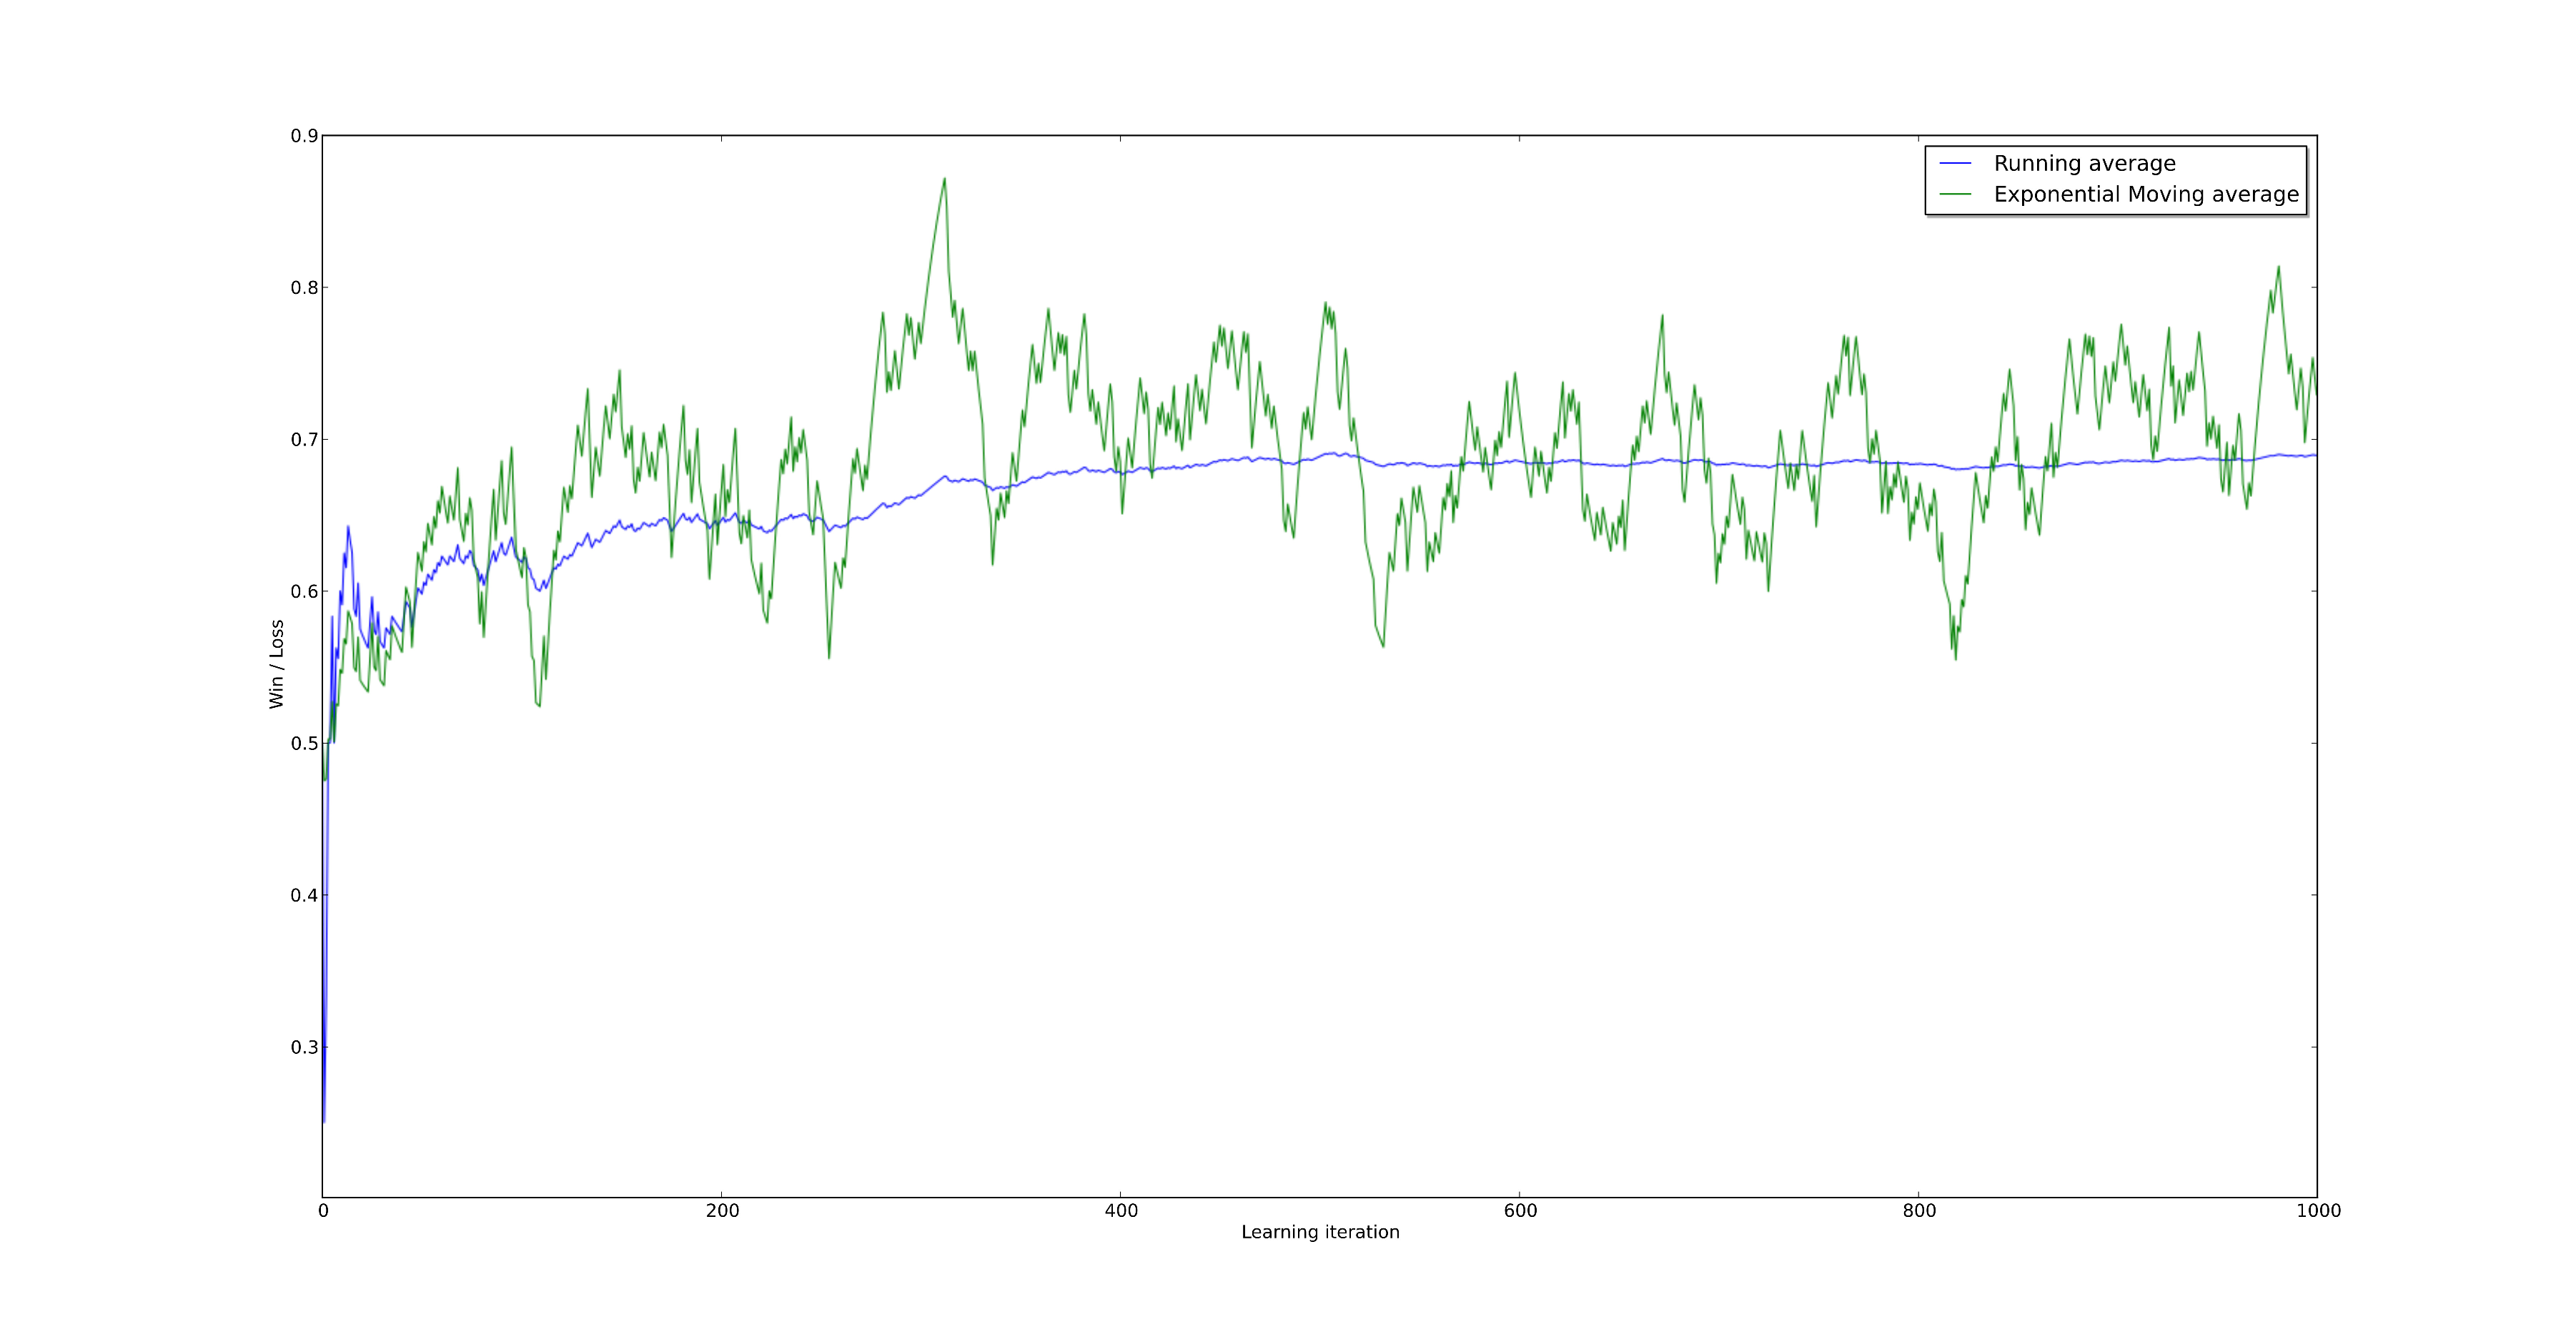
\includegraphics[trim= 6cm 2cm 5.5cm 3cm, clip,width=1\textwidth]{../Graphs/Learning_2ply_First1000.pdf}
  \caption{Learning Progress of a 4-ply Learning player vs. a 4-ply Minimax
    player}
  \label{LearningProgress}
\end{figure}

\subsection{Staged Learning}
\label{sec:staging}

Jafar performs \tdl\ learning in \emph{stages}. Each stage defines a separate
set of feature weights for a certain number of moves in the game. This allows
the agent to play with alternate strategies at different points throughout the
game, for example playing conservatively and leaving options open early game
and changing to a greedier nature near the end. In the most extreme case we
can split the agent into 92 game stages, maintaining a different set of
feature weights for every move of the game.

However, each stage we add to the agent corresponds to a linear increase in
the number of parameters \tdl\ must learn. This possibly leads to an
exponential increase in convergence time for the algorithm.  In
Figure~\ref{WeightsOverTime} and Figure~\ref{WeightsOverTime92} below we see
show the feature weights throughout the game for a 20-stage and 92-stage
version of Jafar; with \tdl\ run over 1000 and 30000 games respectively.

Notice that the two graphs are for the most part very similar; we see all the
same trends in both (though the 92-stage agent shows these trends in greater
detail). Note that the 20-stage agent has been running for a thirtieth the
amount of time that the 92-stage agent has; and the fact that the results are
similar reflects our above intuition regarding the increase in learning time
required.

Both agents below exhibit excessive `zig-zagging' (more notably in the
92-stage agent). This effect occurs due to the \emph{parity} of the board:
optimal play style differs slightly depending on whether or not the
agent will take the last move of the game. This effect is still observable in
the 20-stage agent since the stages have a differing amount of odd and even
parity moves.

%Hrmmmm looks good but really needs to be consistent with 92-stager. So need to
%rollback or tikzify both (or could fix colours here and axes below?)
\begin{figure}[htbp]
  \centering
  \begin{tikzpicture}
    \begin{axis}[width=0.75\textwidth, height=0.5\textwidth,
      xlabel=Stage, ylabel=Feature Weight, legend columns=2,
      ytick={0, 0.1, 0.2, 0.3, 0.4, 0.5},
      no markers, enlargelimits=false, ymin=0, ymax=0.5]
      \addplot table[x=stage, y=LM] {../Graphs/Weights_Over_Time_20.txt};
      \addlegendentry{Legal Moves}
      \addplot table[x=stage, y=SC] {../Graphs/Weights_Over_Time_20.txt};
      \addlegendentry{Stone Count}
      \addplot table[x=stage, y=BA] {../Graphs/Weights_Over_Time_20.txt};
      \addlegendentry{Blocked Adjacent}
      \addplot table[x=stage, y=SP] {../Graphs/Weights_Over_Time_20.txt};
      \addlegendentry{Side Pieces}
      \addplot table[x=stage, y=CP] {../Graphs/Weights_Over_Time_20.txt};
      \addlegendentry{Corner Pieces}
    \end{axis}
  \end{tikzpicture}
  \caption{Learned weights for a 20-stage player after 1000 learning
    iterations}
  \label{WeightsOverTime}
\end{figure}

\begin{figure}[htbp]
  \centering
  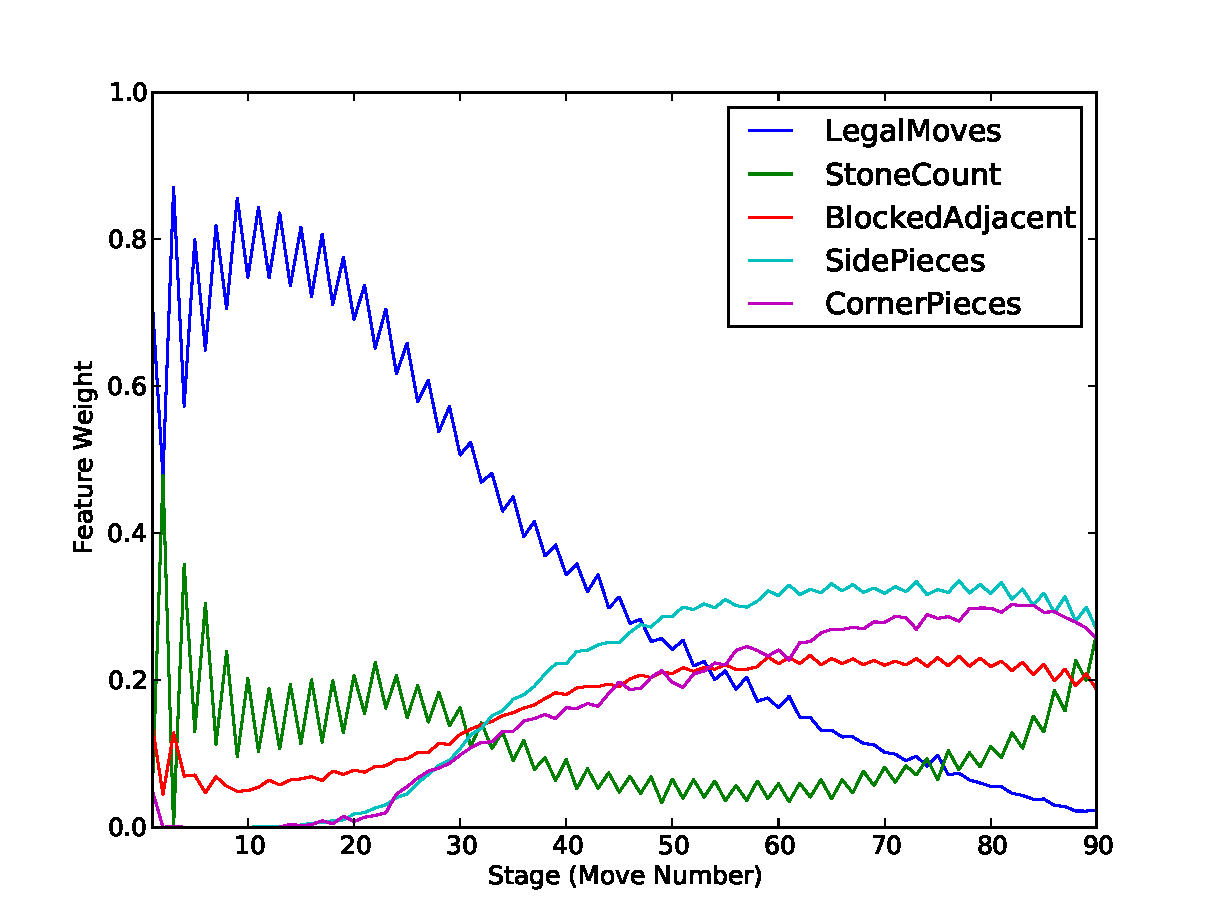
\includegraphics[trim=0cm 0cm 1.5cm 1cm, clip, width=0.75\textwidth]
    {../Graphs/finalweights.pdf}
  \caption{Learnt weights for a 92-stage player, after 30000 learning iterations}
  \label{WeightsOverTime92}
\end{figure}


\begin{figure}[H]
  \centering
  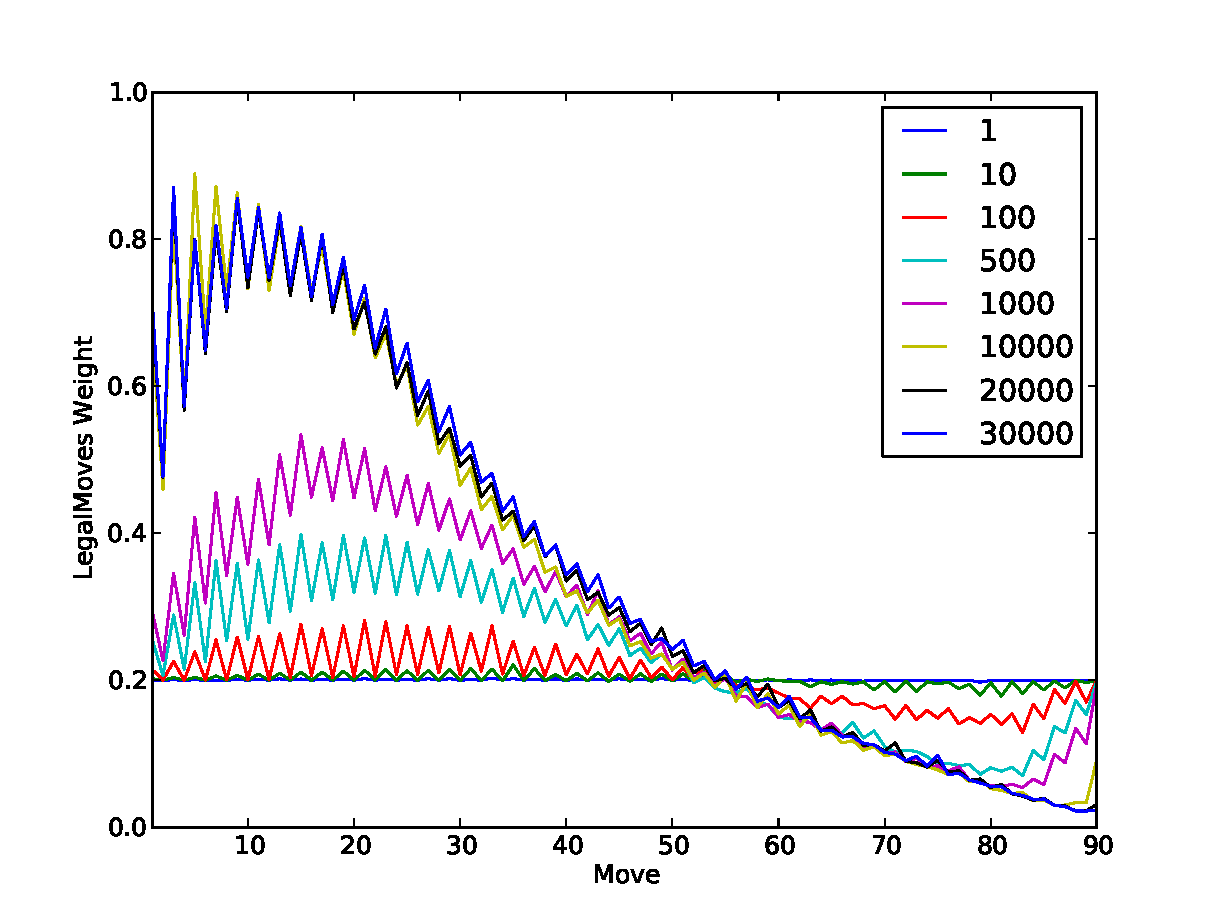
\includegraphics[trim=0cm 0cm 1.5cm 1cm, clip, width=0.75\textwidth]
    {../Graphs/legalmovesprogression.pdf}
  \caption{The LegalMoves feature weights converging over time}
  \label{LegalMovesConvergence}
\end{figure}

Figure~\ref{LegalMovesConvergence} shows us the convergence of the 92-stage agent
over time (for a single feature weight). Notice that there is very little
change after about 10000 games; implying that the agent has converged. Compare this
with the 20-stage agent above, who achieves a similar level of convergence after 1000
games.


\subsection{ELO Arena}
\label{sub:elo_arena}

While \tdl\ provides a exceedingly \emph{efficient} method of learning feature weights,
it is by no means \emph{intuitive}; in the sense that the learning process occurs
entirely within a mathematical formula. Thus we developed the \emph{ELO Arena};
a genetic algorithm entirely of our own design which serves to cross-validate
\tdl\ and more intuitively demonstrate learning.

The ELO Arena starts by generating a set of agents with random feature weights.
These agents then compete against each other for ELO rating points. The ELO rating
system was designed by Arpad Elo as a method of ranking international Chess players.
In the ELO Arena these rating points keep track of the relative skill levels of the competing
agents.

After each of the random agents have played a fixed number of games (and had their
ratings updated accordingly) a new agent is introduced. This new agent bases its feature
weights off of the current top 5 rated players in the following manner:
\begin{enumerate}
\item Take a weighted average of the feature weights from the top 5 players
\item \emph{Mutate} these weights by adding a random low-variance Gaussian variable
\end{enumerate}

Over time we should observe that agents with good mutations float to the top of the rating system.
This should lead to our new agents performing better and better until eventually
converging to weights similar to those learnt by \tdl.

\subsection{Comparison of \tdl\ and ELO arena}
\label{sub:comparing_learning}
%% TD lambda and ELO arena

\section{Performance evaluation}
\label{sec:performance}
%% Tournament results, self play learning, fixed opponent results.

\section{Improvements}
\label{sec:improvements}
%% Look at the performance and say what we could have improved.

\section{Final Comments}
\label{sec:final_comments}


\bibliographystyle{chicago}
\bibliography{ai}
\end{document}
